\section{Tests}
In this section, we present two sets of test cases to validate the results we obtained with the formulations we derived. The first case is the biaxial tension test which is used to calibrate material constants. For isotropic materials, the analytical solution is easy to find if we assume the material is incompressible. The second case is the expansion of a vessel, which is a very representative application in the field of biomechanics.  

\subsection{Biaxial Tension Test}
\label{biaxial_tension_test}
A long bar loaded equally in two directions with fixed tractions is considered. The section of the bar is a $1$ $m^2$ square. As shown in Figure \ref{fig:biaxial_schematic}, the bottom surface is fixed in $z$-direction; the left surface is fixed in $y$-direction and the back surface is fixed in $x$-direction. External tractions are applied to the front and right surfaces. Define the stretch $\lambda$ as the ratio between the deformed length to the original length, then for isotropic incompressible material, the stress is expressed as:
\begin{equation}
S_{11} = S_{22} = 2(1 - {\lambda}^{-6})(\frac{\partial\Psi_{iso}}{\partial\bar{I}_1} + {\lambda}^2\frac{\partial\Psi_{iso}}{\partial\bar{I}_2}), \quad S_{33} = 0
\end{equation}
where $S_{11}$, $S_{22}$, $S_{33}$ are the diagonal components of the PK2 stress, all the off-diagonal components are $0$.

Denote the nonzero component of PK2 stress as $S$. For Mooney-Rivlin model, plug in Equation \ref{iso1}, we have

\begin{equation}
S = (1 - {\lambda}^{-6})(\mu_1 + \mu_2{\lambda}^2)
\end{equation}
and therefore the nominal stress $P$ is
\begin{equation}
P = \lambda S =  (\lambda - {\lambda}^{-5})(\mu_1 + \mu_2{\lambda}^2)
\end{equation}
Neglecting the $\mu_2$ terms we have the nominal stresse for Neo-Hookean model
\begin{equation}
P = \lambda S =  \mu_1(\lambda - {\lambda}^{-5})
\end{equation}
Similarly, for Yeoh model
\begin{equation}
P = \lambda S = 2(\lambda - {\lambda}^{-5})[c_1 + 2c_2(2{\lambda}^2 + {\lambda}^{-4} - 3) + 3c_3(2{\lambda}^2 + {\lambda}^{-4} - 3)^2]
\end{equation}

\begin{figure}[h!]
\centering
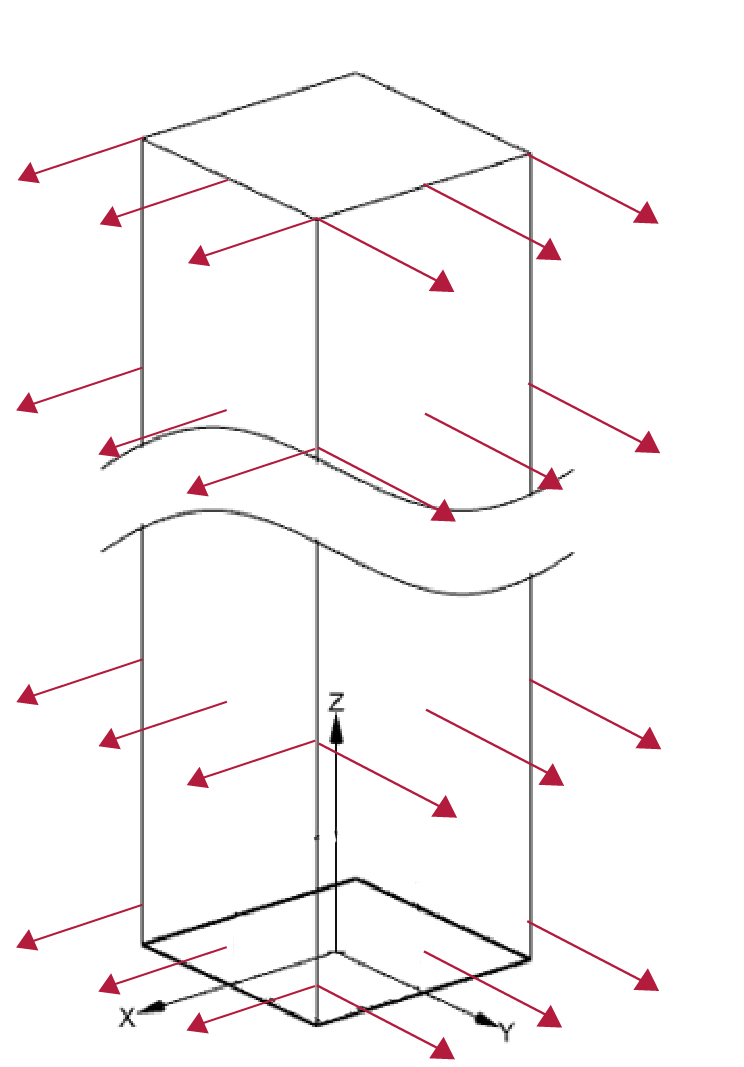
\includegraphics[width=.3\textwidth]{./figures/biaxial_schematic.jpg}
\caption{Schematic Diagram of Biaxial Tension Test}
\label{fig:biaxial_schematic}
\end{figure}

The material constants used in these models are curve-fitted from the standard ASTM412 tensile test results of the same material. See Shashikant. In Neo-Hookean model, $\mu_1 = 0.6548$ MPa; in Mooney-Rivlin model, $\mu_1 = 0.595522$ MPa, $\mu_2 = 0.050381$ MPa; in Yeoh model, $c_1 = 0.358756$ MPa, $c_2 = - 0.0508009$ MPa, $c_3 = 0.0142132$ MPa. The Poisson's ratios for all the models are over $\nu = 0.49999$, closed enough to incompressibility.

Figure \ref{fig:biaxial1} shows the results of the theoretical calculation and numerical computation. Perfect agreement is achieved. As expected, in the small strain range, all these models have similar linear performance. Also, it can be seen that $\mu_2$ in Mooney-Rivlin model acts as a modification to $\mu_1$ in Neo-Hookean model which increases the stiffness. In large strain range, the stiffness of Yeoh model grows quickly, becoming significantly larger than the others.

\begin{figure}[h!]
\centering
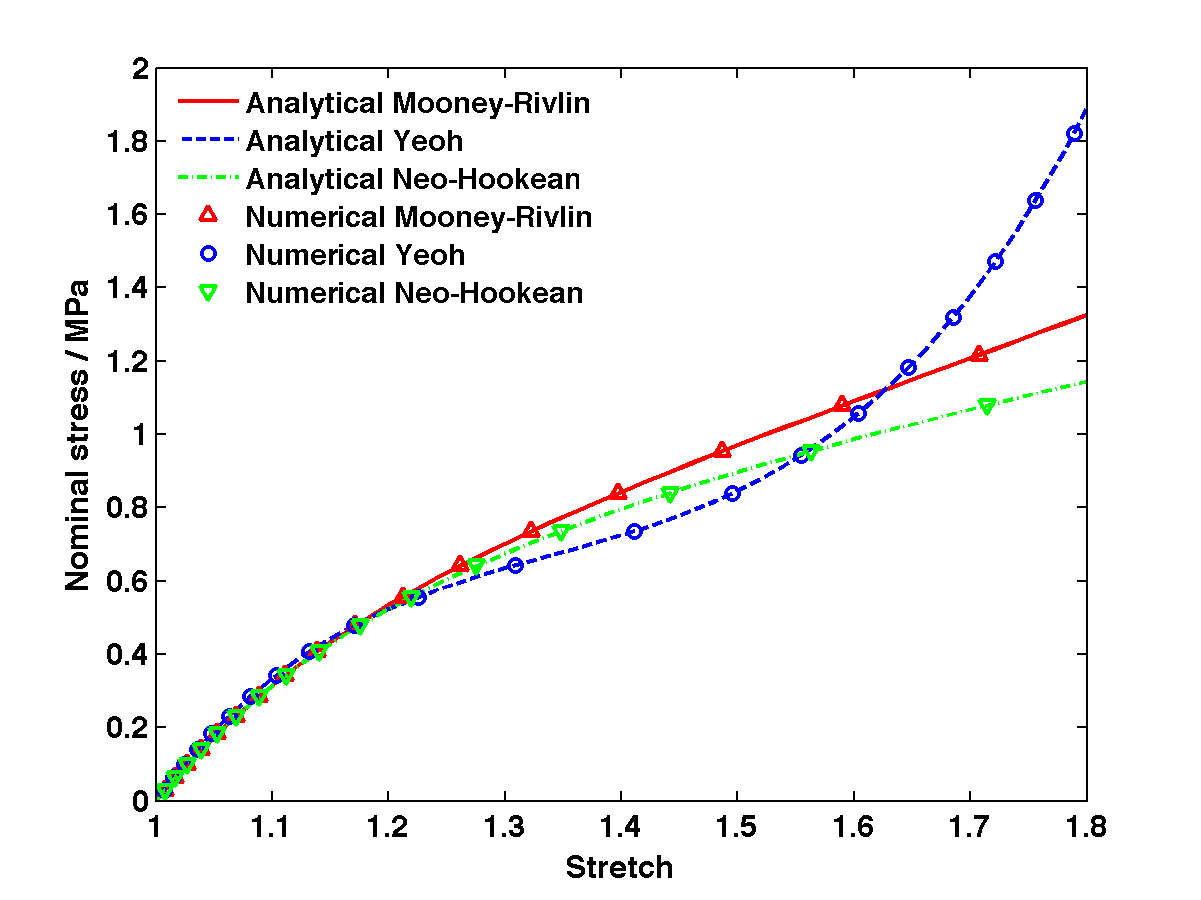
\includegraphics[width=.6\textwidth]{./figures/biaxial1.png}
\caption{Biaxial Tension Test for Isotropic Models}
\label{fig:biaxial1}
\end{figure}

To demonstrate the anisotropy of HGO model, we compare the stretches in two directions in the biaxial tension test. We use the material parameters calibrated from the media layer of artery in [ ] but only one direction is strengthened. That is, both two families of fibers are arranged in the same direction. The material parameters are $\mu_1 = 3$ KPa, $k_1 = 2.3632$ KPa and $k_2 = 0.8393$. We change the direction of the fibers which measured by the angle from the $x$ direction denoted as $\alpha$. 

We define the stretch ratio $\lambda$ in Equation \ref{stretchratio}, and plot the stretch ratio against the nominal stress in Figure \ref{fig:biaxial2}. Just as what we expect, the stretch ratio at $\alpha = 0^\circ$ is the same as $\alpha = 90^\circ$, and similarly for $\alpha = 30^\circ$ and $\alpha = 60^\circ$. 
$\lambda_y$ is greater than $\lambda_x$ when $0^\circ < \alpha < 45^\circ$ since the $x$ direction is strengthened more. As the angle gets larger, $\lambda_x$ becomes greater too. While $\alpha = 45^\circ$ two directions become symmetric again.

\begin{equation}
\label{stretchratio}
\lambda = 
\begin{cases}
	\lambda_y/\lambda_x, & \text{$\alpha = 0^\circ$, $30^\circ$ or $45^\circ$} \\
	\lambda_x/\lambda_y, & \text{$\alpha = 60^\circ$ or $90^\circ$}
\end{cases}
\end{equation}
 
\begin{figure}[h!]
\centering
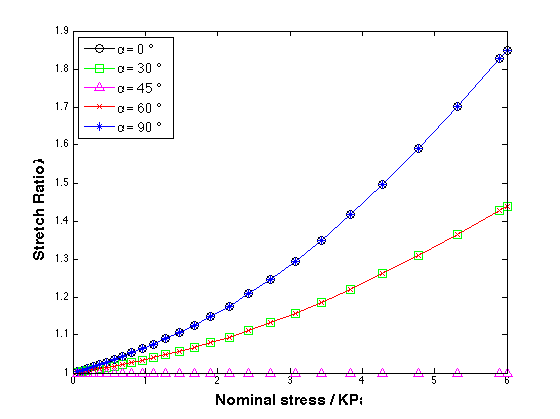
\includegraphics[width=.6\textwidth]{./figures/biaxial2.png}
\caption{Biaxial Tension Test for HGO Model}
\label{fig:biaxial2}
\end{figure}

\subsection{Cylindrical Pressure Vessel}
\label{pressure_vessel}
As a typical application, we consider a vessel under lumen pressure. The vessel has an internal radius of $R_i = 7$ m and an external radius of $R_o = 18.625$ m. Only a quarter of vessel is considered with plain strain assumption as shown in Figure \ref{fig:vessel_schematic}. $21$ nodes are uniformly distributed in radial direction. As the first case, we model the vessel with Mooney-Rivlin model. The material parameters used are $\mu_1 = 160$ MPa and $\mu_2 = 40$ MPa. $\kappa$ is set to $1 \times 10^7$ MPa to make the material nearly incompressible. We compare the radial displacement, hoop stress, radial stress, and axial stress with the analytical solutions of incompressible Mooney-Rivlin model under an internal pressure of $p_i = 50$ MPa. The analytical solutions are found in [] as follows 
\begin{subequations}
\begin{align}
p_i &= 2(\mu_1 + \mu_2)(log\frac{{R_i}^2 + b}{{R_o}^2 + b} - 2log\frac{R_i}{R_o} +
b\frac{{R_o}^2 - {R_i}^2}{({R_o}^2+b)({R_i}^2+b)}) \\
u_r &= -R + \sqrt{R^2 + b} \\
p &= - p_i - \mu_2 - (\mu_1 + \mu_2)(log\frac{r}{R_i} + \frac{b}{2}(r^2 - {R_i}^2) - log\frac{R}{R_i} + {(\frac{R_i}{r})}^2) ) \\
\sigma_{\theta} &= p + \mu_2 + (\mu_1 + \mu_2)(\frac{r}{R})^2 + C \\
\sigma_r &= p + \mu_2 + (\mu_1 + \mu_2)(\frac{R}{r})^2 + C \\
\sigma_z &= p +  \mu_1 + \mu_2[(\frac{R}{r})^2 + (\frac{r}{R})^2] + C
\end{align}
\end{subequations}
where $R$ and $r$ are the radial coordinate before and after deformation, $p$ is the hydrostatic pressure, $u_r$ is the radial displacement, and $\sigma_{\theta}$, $\sigma_r$ and $\sigma_z$ are the hoop, radial and axial stresses respectively. $b$ is a constant determined by the internal pressure $p_i$, and $C$ is an arbitrary constant since the material is incompressible. 

\begin{figure}[h!]
\centering
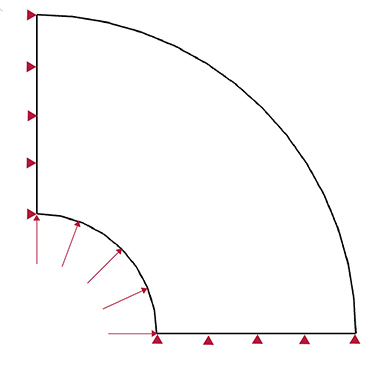
\includegraphics[width=.3\textwidth]{./figures/vessel_schematic.jpg}
\caption{Schematic Diagram of Pressure Vessel}
\label{fig:vessel_schematic}
\end{figure}

Fig \ref{fig:mooney-rivlin1} shows the stress components and the radial displacement along radius direction. Good agreement is achieved on all the components. Notice the axial stress is usually hard to predict but our result is satisfactory. Furthermore, we pick the node at the midpoint in the radial direction ($R = 12.8125$ m) and study its deformation under different internal pressures. As shown in Fig \ref{fig:mooney-rivlin2}, the computational result and analytical solution agree perfectly with each other. 

\begin{figure}[t!p]
	\begin{subfigure}[b]{0.5\textwidth}
		\centering
		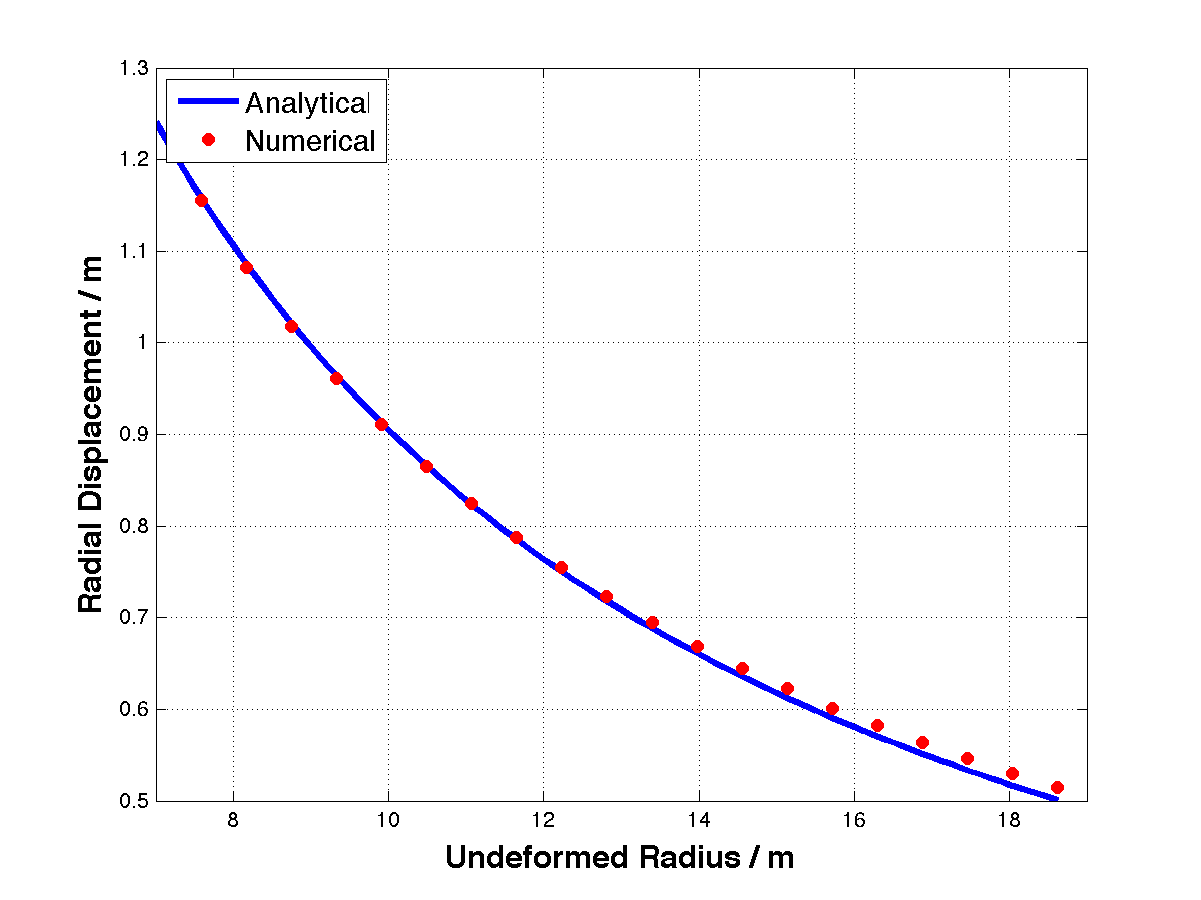
\includegraphics[width=\textwidth]{./figures/ur_50.png}
		\caption{Radial Displacement}
		\label{ur_50}
	\end{subfigure}
	\begin{subfigure}[b]{0.5\textwidth}
		\centering
		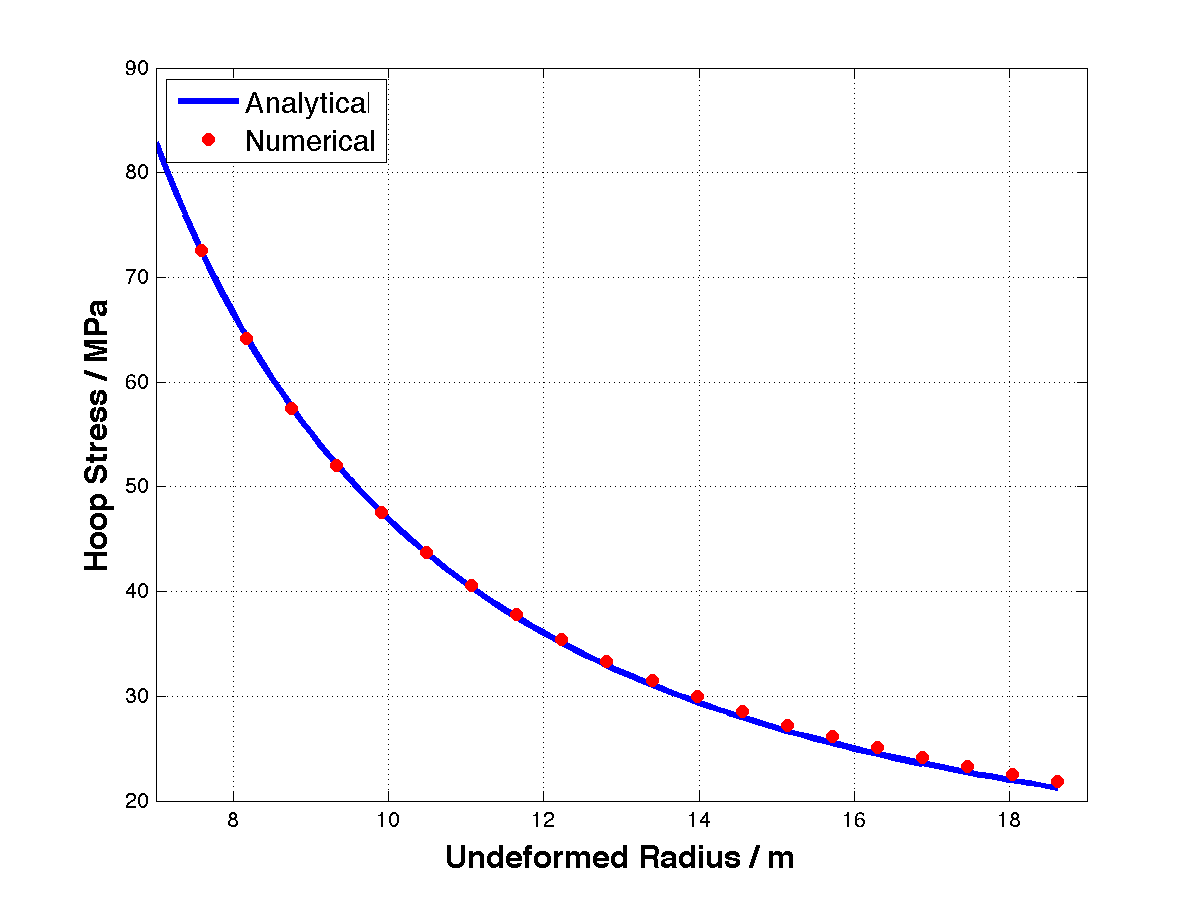
\includegraphics[width=\textwidth]{./figures/hoop_stress_50.png}
		\caption{Hoop Stress}
		\label{hoop_50}
	\end{subfigure}
	
	\begin{subfigure}[b]{0.5\textwidth}
		\centering
		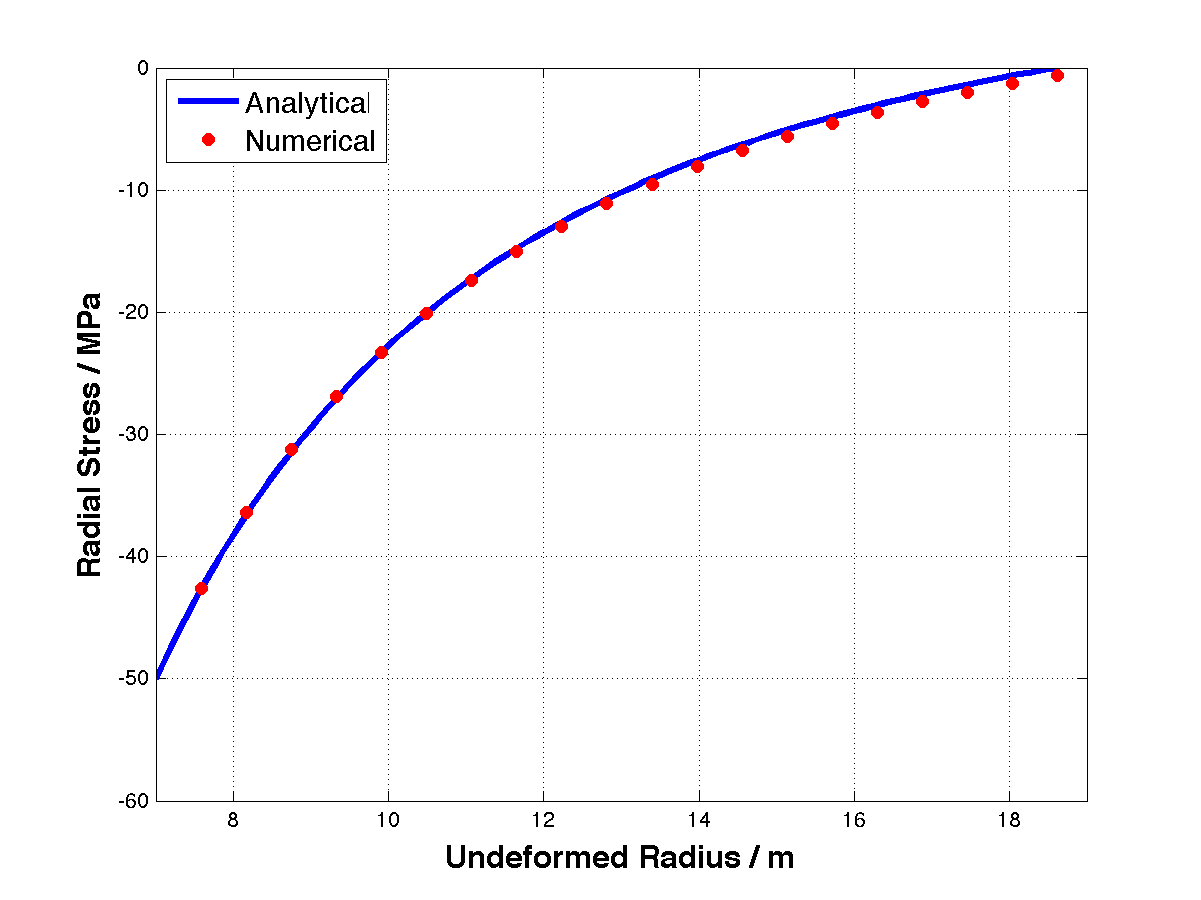
\includegraphics[width=\textwidth]{./figures/radial_stress_50.png}
		\caption{Radial Stress}
		\label{radial_50}
	\end{subfigure}
	\begin{subfigure}[b]{0.5\textwidth}
		\centering
		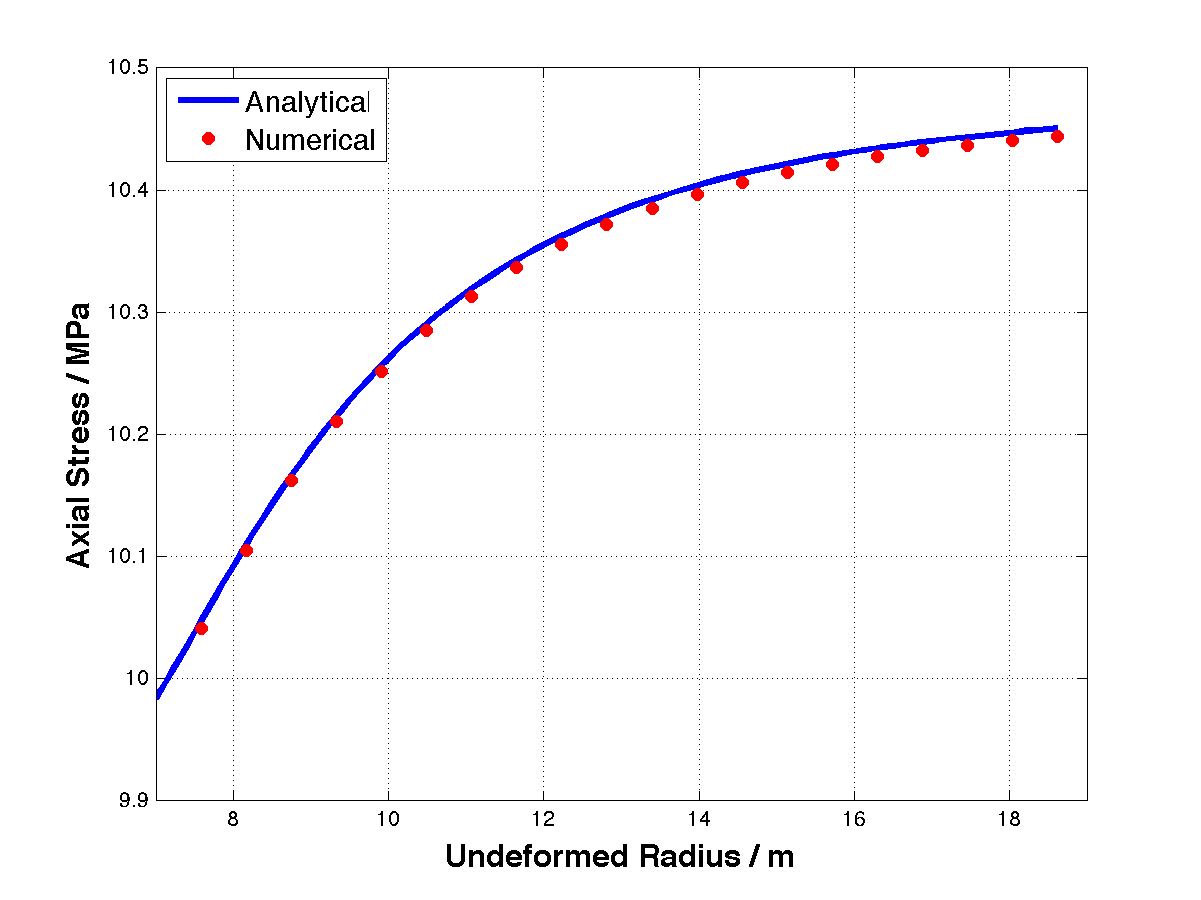
\includegraphics[width=\textwidth]{./figures/axial_stress_50.png}
		\caption{Axial Stress}
		\label{axial_50}
	\end{subfigure}
	\caption{Vessel Expansion Under $p_i = 50$ MPa with Mooney-Rivlin Model}
	\label{fig:mooney-rivlin1}
\end{figure}

\begin{figure}[t!p]
	\begin{subfigure}[b]{0.5\textwidth}
		\centering
		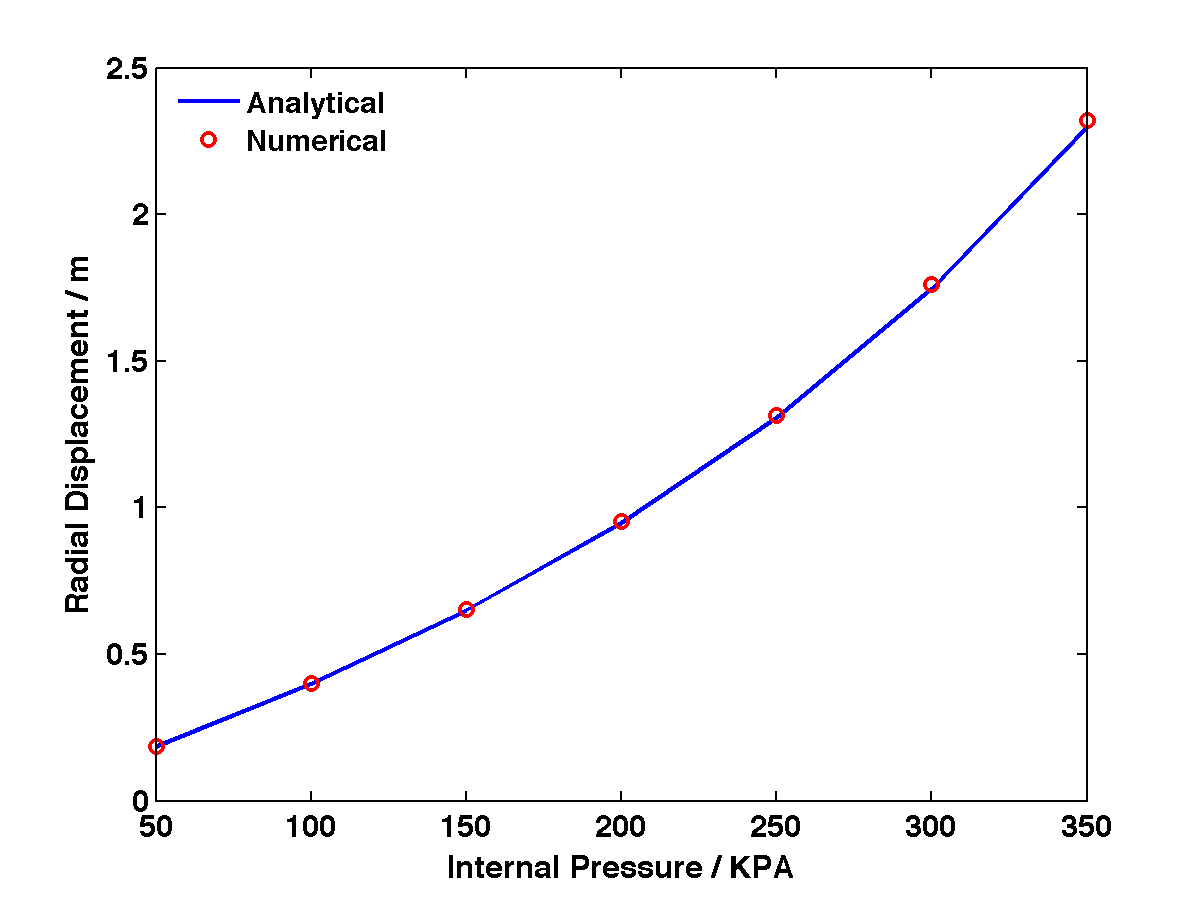
\includegraphics[width=\textwidth]{./figures/ur.png}
		\caption{Radial Displacement}
		\label{ur}
	\end{subfigure}
	\begin{subfigure}[b]{0.5\textwidth}
		\centering
		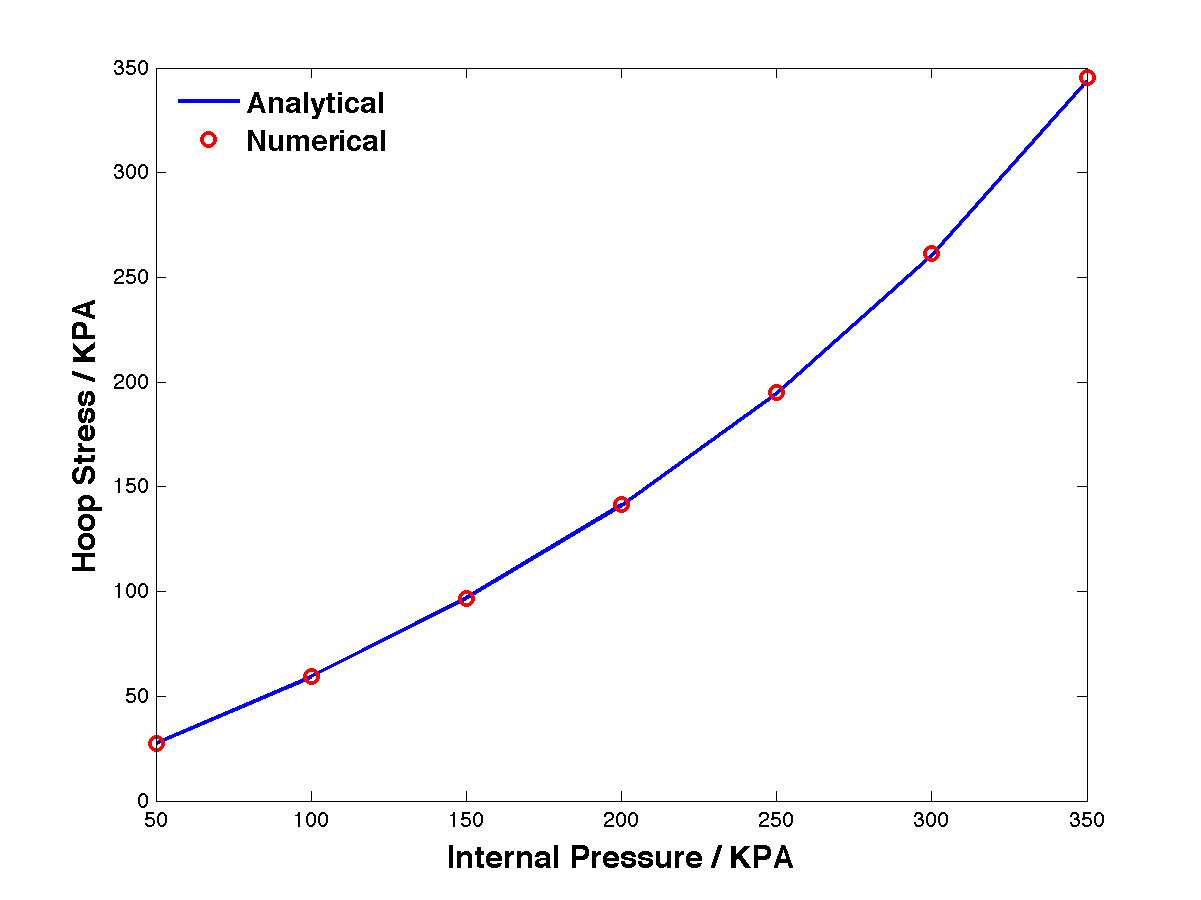
\includegraphics[width=\textwidth]{./figures/hoop.png}
		\caption{Hoop Stress}
		\label{hoop}
	\end{subfigure}
	
	\begin{subfigure}[b]{0.5\textwidth}
		\centering
		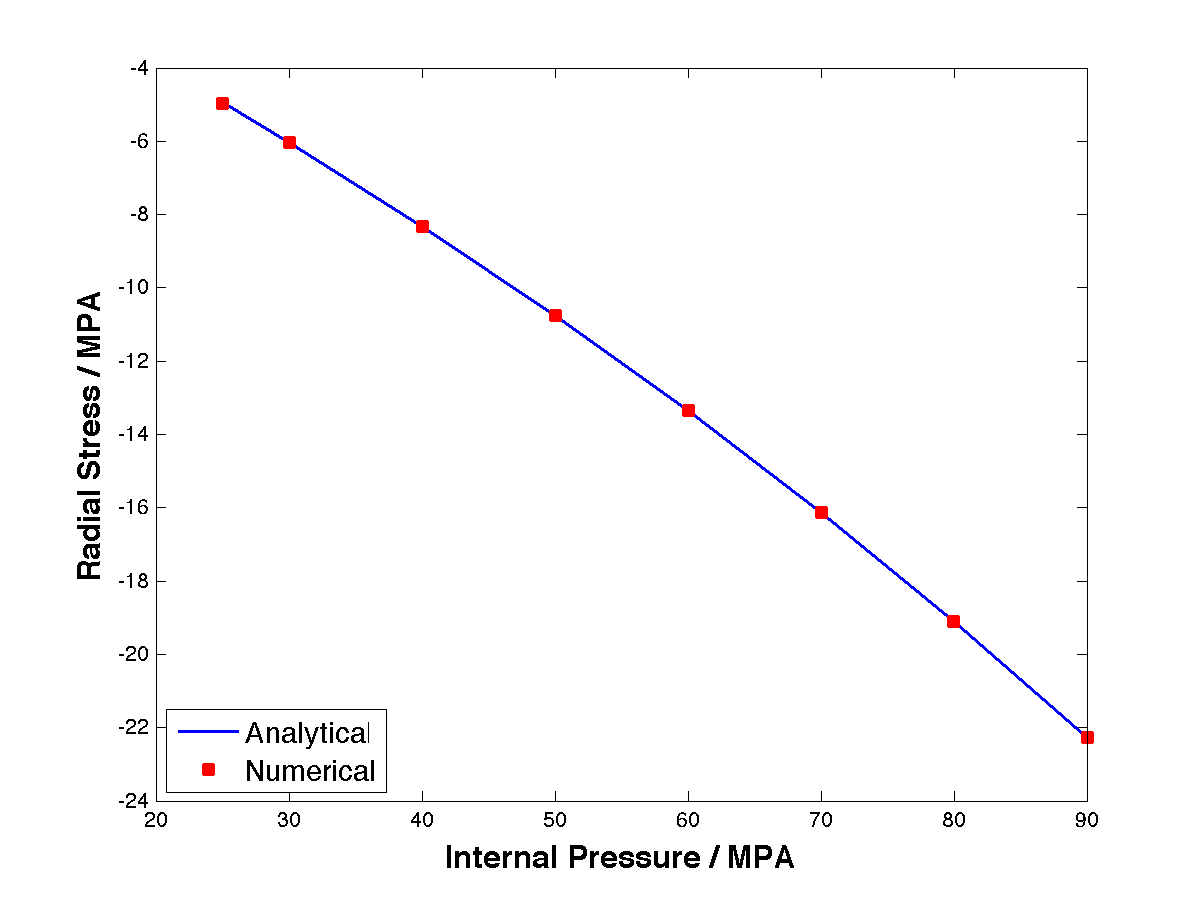
\includegraphics[width=\textwidth]{./figures/radial.png}
		\caption{Radial Stress}
		\label{radial}
	\end{subfigure}
	\begin{subfigure}[b]{0.5\textwidth}
		\centering
		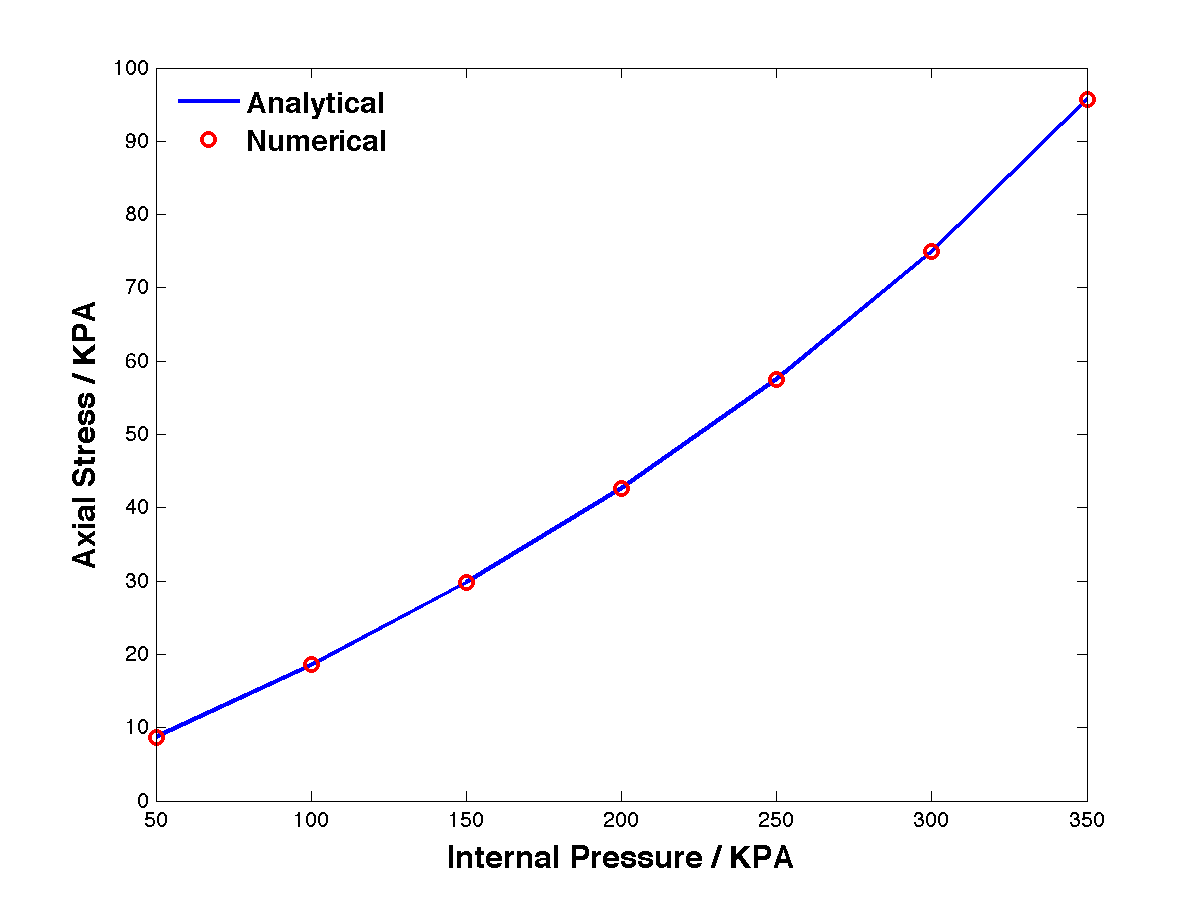
\includegraphics[width=\textwidth]{./figures/axial.png}
		\caption{Axial Stress}
		\label{axial}
	\end{subfigure}
	\caption{Vessel Expansion Under Different Pressure with Mooney-Rivlin Model}
	\label{fig:mooney-rivlin2}
\end{figure}

Next we use Neo-Hookean and Yeoh model to characterize the same material and repeat the vessel expansion test. The material constants are the same as in Section \ref{biaxial_tension_test}. Figure \ref{hoop_nh_yeoh} shows the results of these two models under an inner pressure of $p_i = 350$ KPa. The displacements have similar trends but different values. It is surprising that hoop stress and radial stress predicted by two models are close. The major difference is the axial stress where Yeoh model predicts a larger range.

\begin{figure}[t!p]
	\begin{subfigure}[b]{0.5\textwidth}
		\centering
		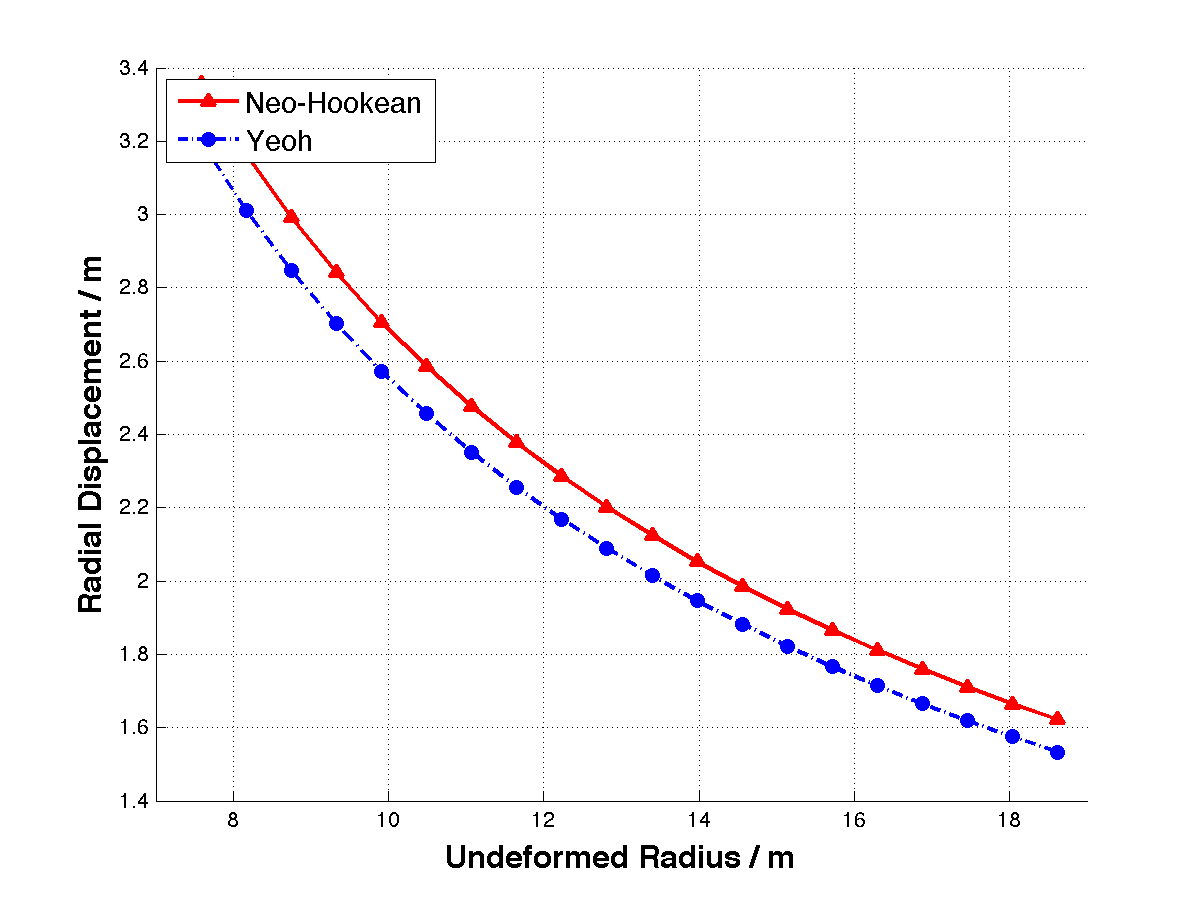
\includegraphics[width=\textwidth]{./figures/ur_nh_yeoh.png}
		\caption{Radial Displacement}
		\label{ur_nh_yeoh}
	\end{subfigure}
	\begin{subfigure}[b]{0.5\textwidth}
		\centering
		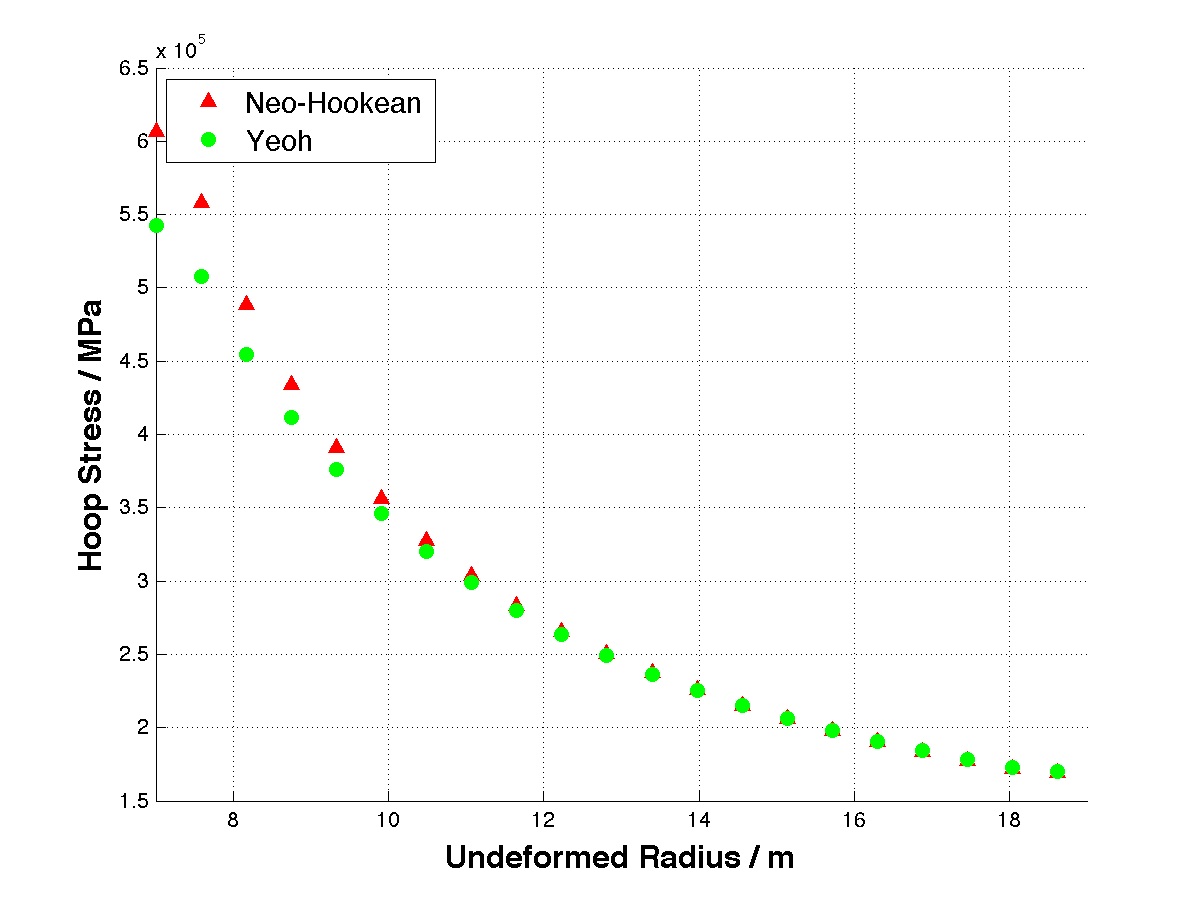
\includegraphics[width=\textwidth]{./figures/hoop_nh_yeoh.png}
		\caption{Hoop Stress}
		\label{hoop_nh_yeoh}
	\end{subfigure}
	
	\begin{subfigure}[b]{0.5\textwidth}
		\centering
		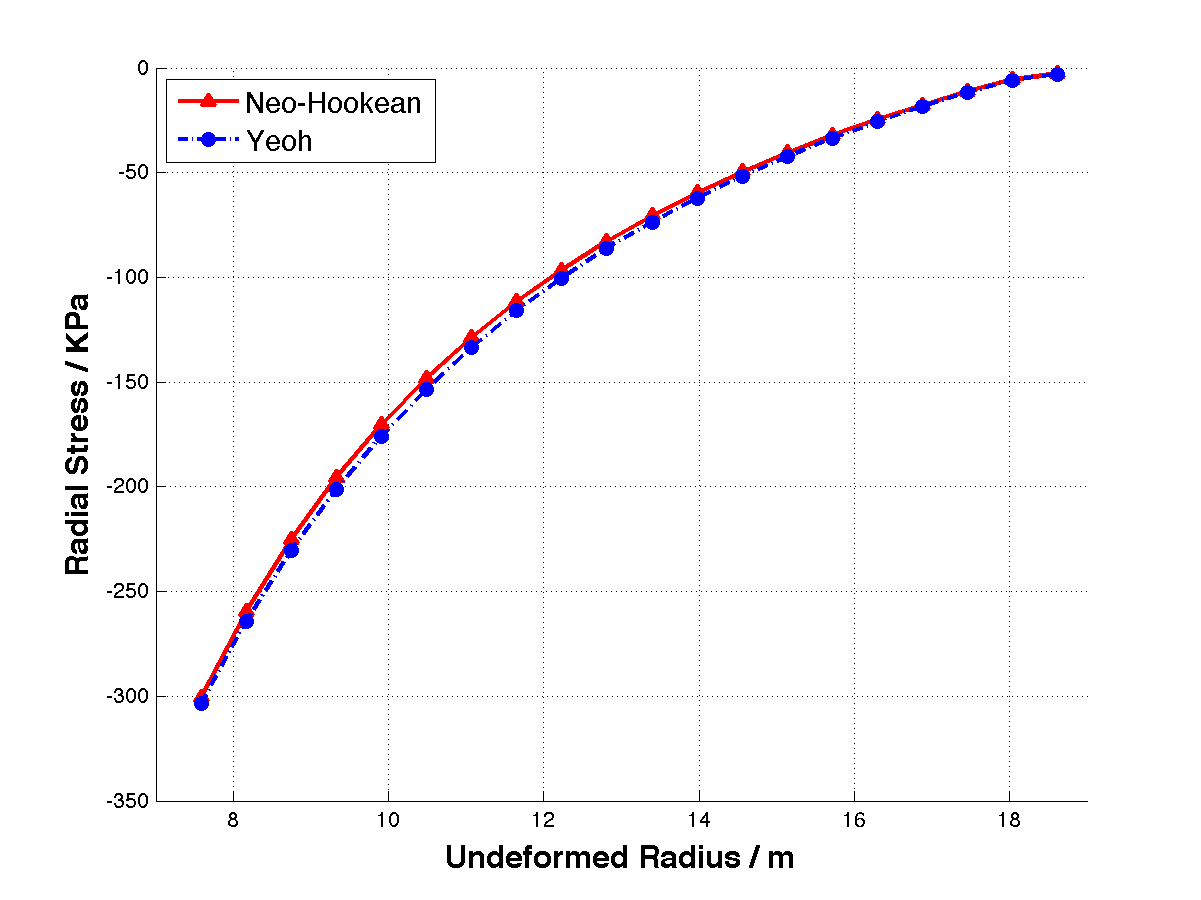
\includegraphics[width=\textwidth]{./figures/radial_nh_yeoh.png}
		\caption{Radial Stress}
		\label{radial_nh_yeoh}
	\end{subfigure}
	\begin{subfigure}[b]{0.5\textwidth}
		\centering
		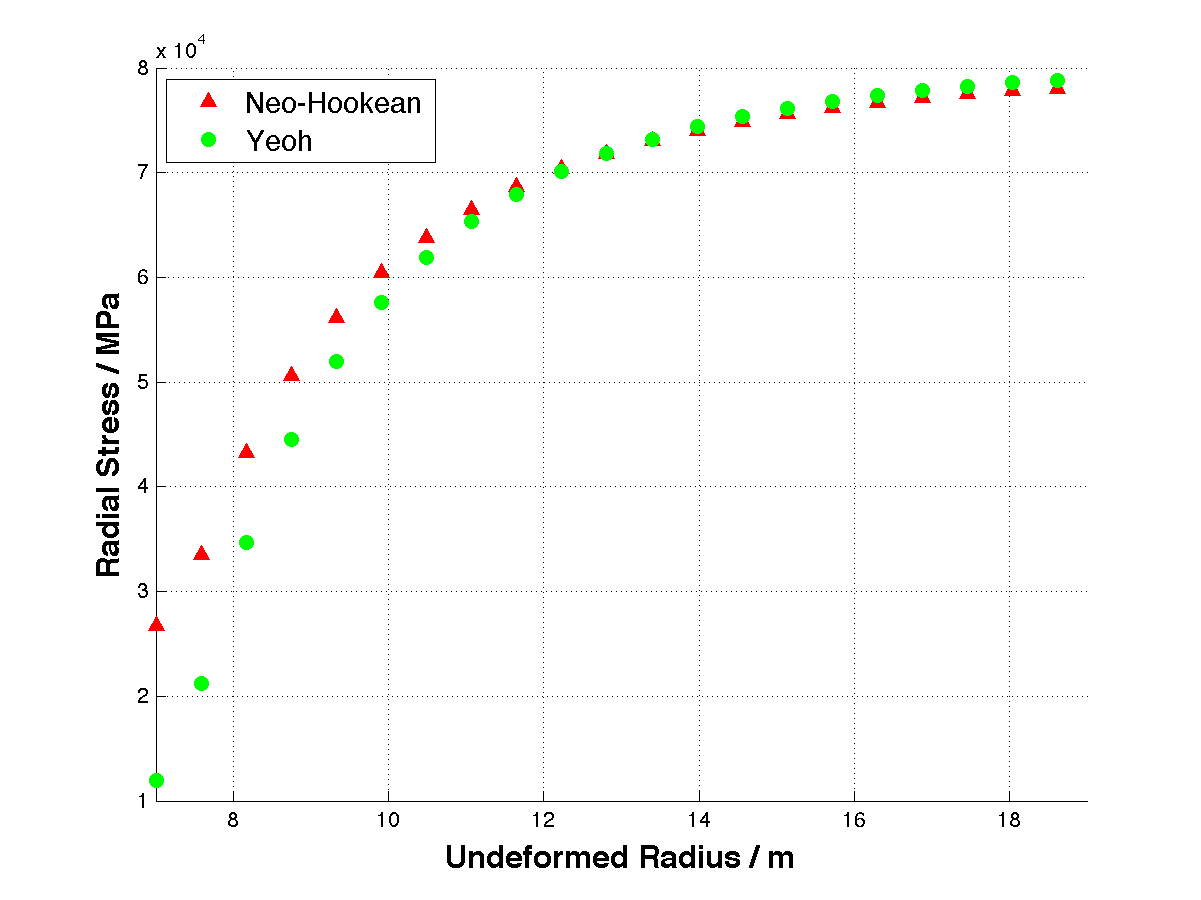
\includegraphics[width=\textwidth]{./figures/axial_nh_yeoh.png}
		\caption{Axial Stress}
		\label{axial_nh_yeoh}
	\end{subfigure}
	\caption{Vessel Expansion with Neo-Hookean and Yeoh Model under $350$ KPa}
	\label{fig:nh_yeoh}
\end{figure}

As the last test case we compare HGO model to Neo-Hookean model. The parameters used in the HGO model is still the same as in Section \ref{biaxial_tension_test}, the geometry and mesh are the same as in previous cases. The pressure is $1.5$ KPa. To demonstrate the effect of the anisotropic part of the HGO model, we use the same $\mu_1$ and $\kappa$ in the Neo-Hookean model. This time, the two families of fibers are arranged in the $\theta-z$ plane with constant angles to the circumferential direction of $\pm 50^\circ$. From Figure \ref{fig:nh_hgo} we can see that overall the vessel is significantly strengthened as the radial displacement is much smaller. While the radial stress does not change much (similar to Yeoh model), the hoop stress is smaller but has a similar trend. However the axial stress changes dramatically. In Neo-Hookean model the inner surface has the maximum axial stress while in HGO model the outer surface has the maximum axial stress. But overall both hoop stress and axial stress are much smaller in the HGO model.

\begin{figure}[t!p]
	\begin{subfigure}[b]{0.5\textwidth}
		\centering
		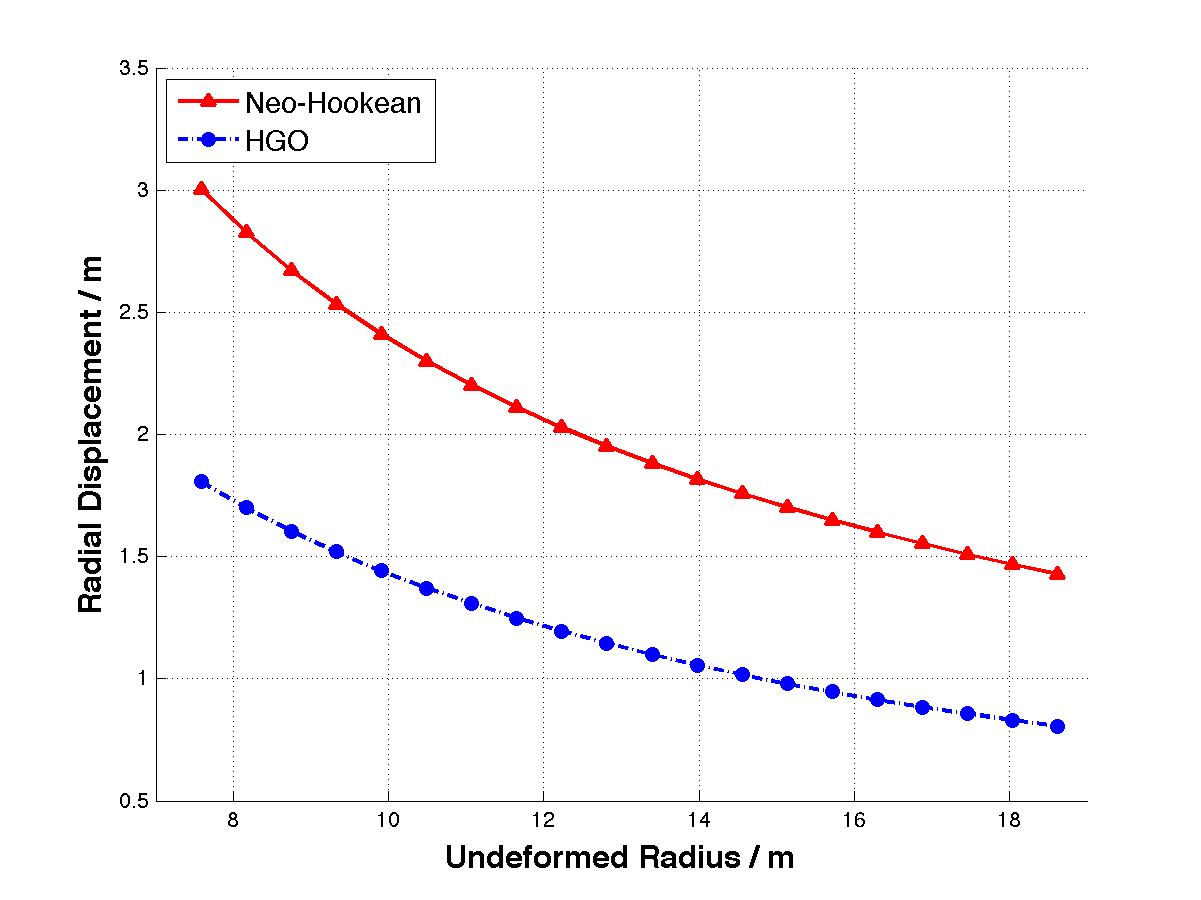
\includegraphics[width=\textwidth]{./figures/ur_nh_hgo.png}
		\caption{Radial Displacement}
		\label{ur_nh_hgo}
	\end{subfigure}
	\begin{subfigure}[b]{0.5\textwidth}
		\centering
		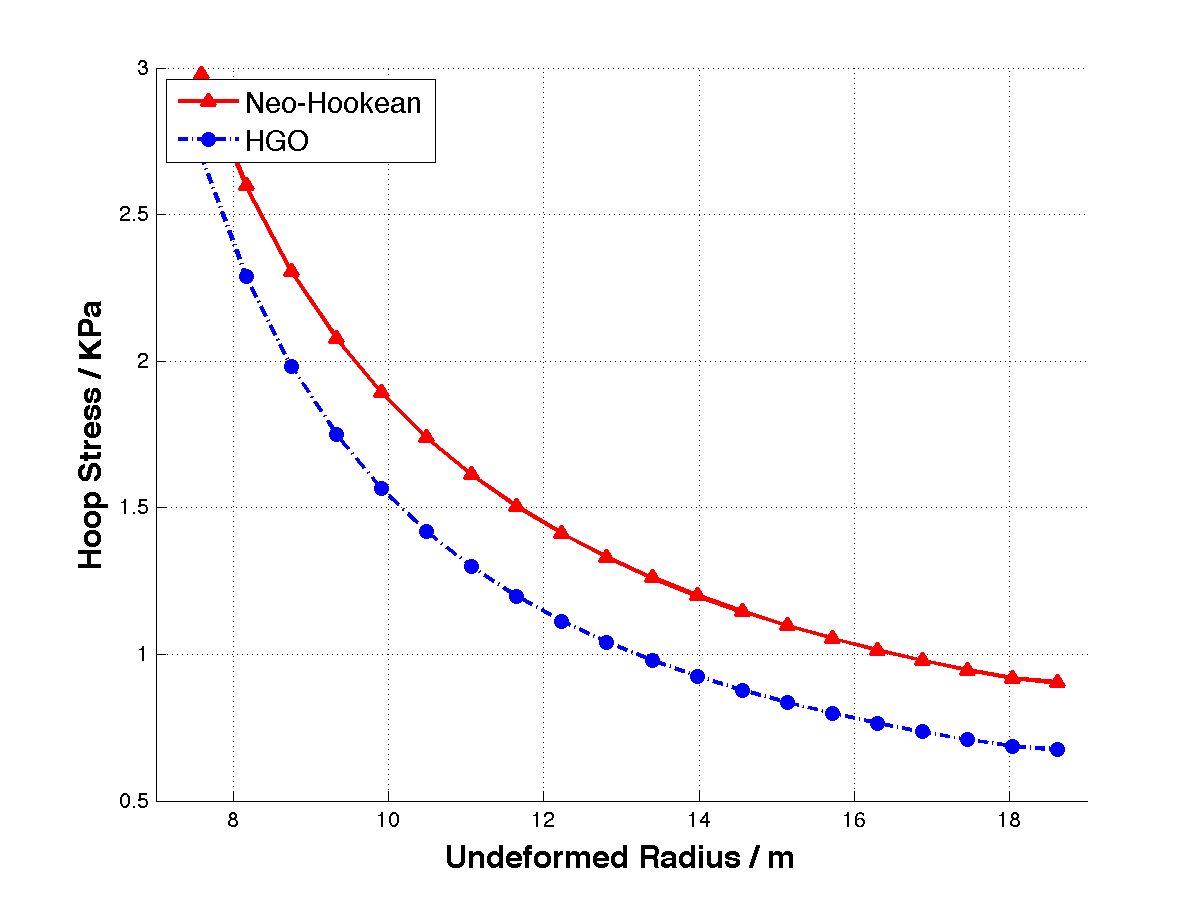
\includegraphics[width=\textwidth]{./figures/hoop_nh_hgo.png}
		\caption{Hoop Stress}
		\label{hoop_nh_hgo}
	\end{subfigure}
	
	\begin{subfigure}[b]{0.5\textwidth}
		\centering
		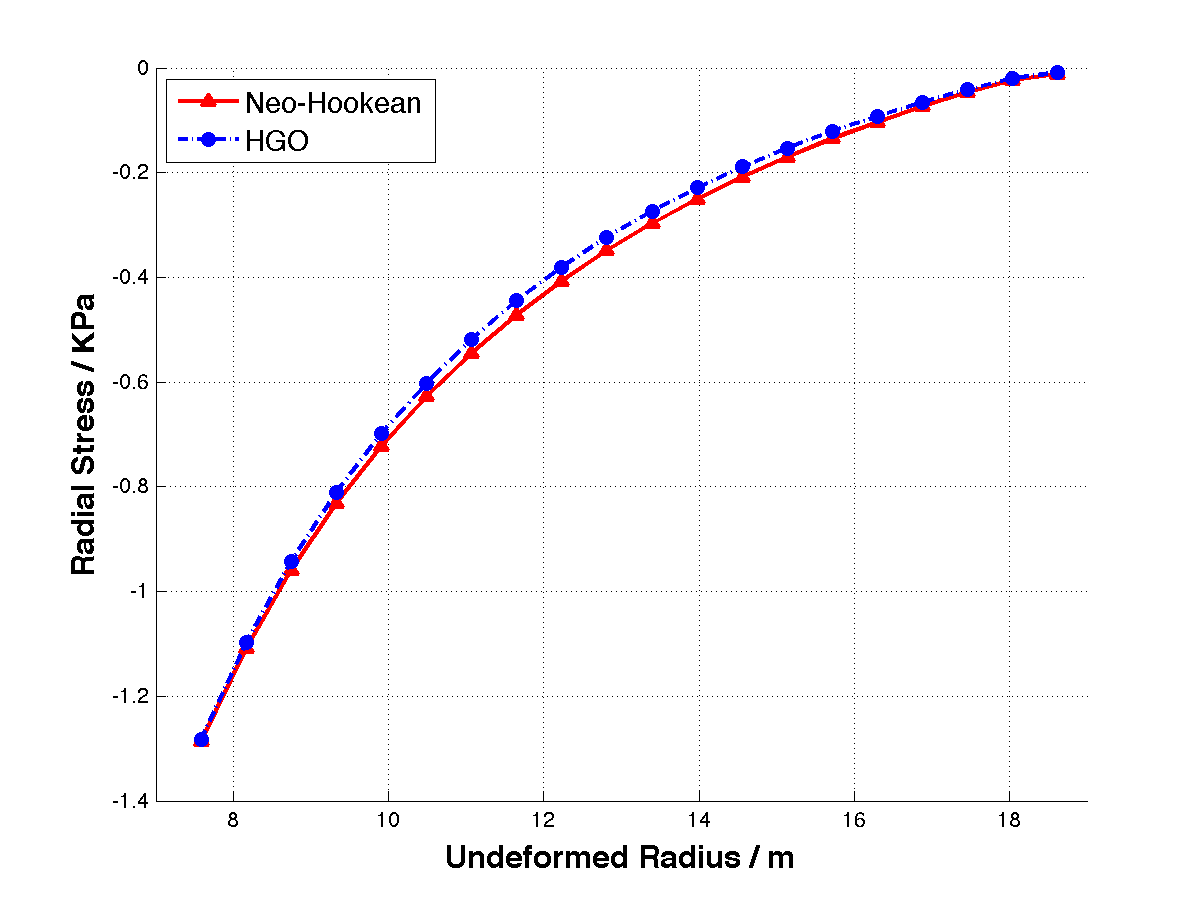
\includegraphics[width=\textwidth]{./figures/radial_nh_hgo.png}
		\caption{Radial Stress}
		\label{radial_nh_hgo}
	\end{subfigure}
	\begin{subfigure}[b]{0.5\textwidth}
		\centering
		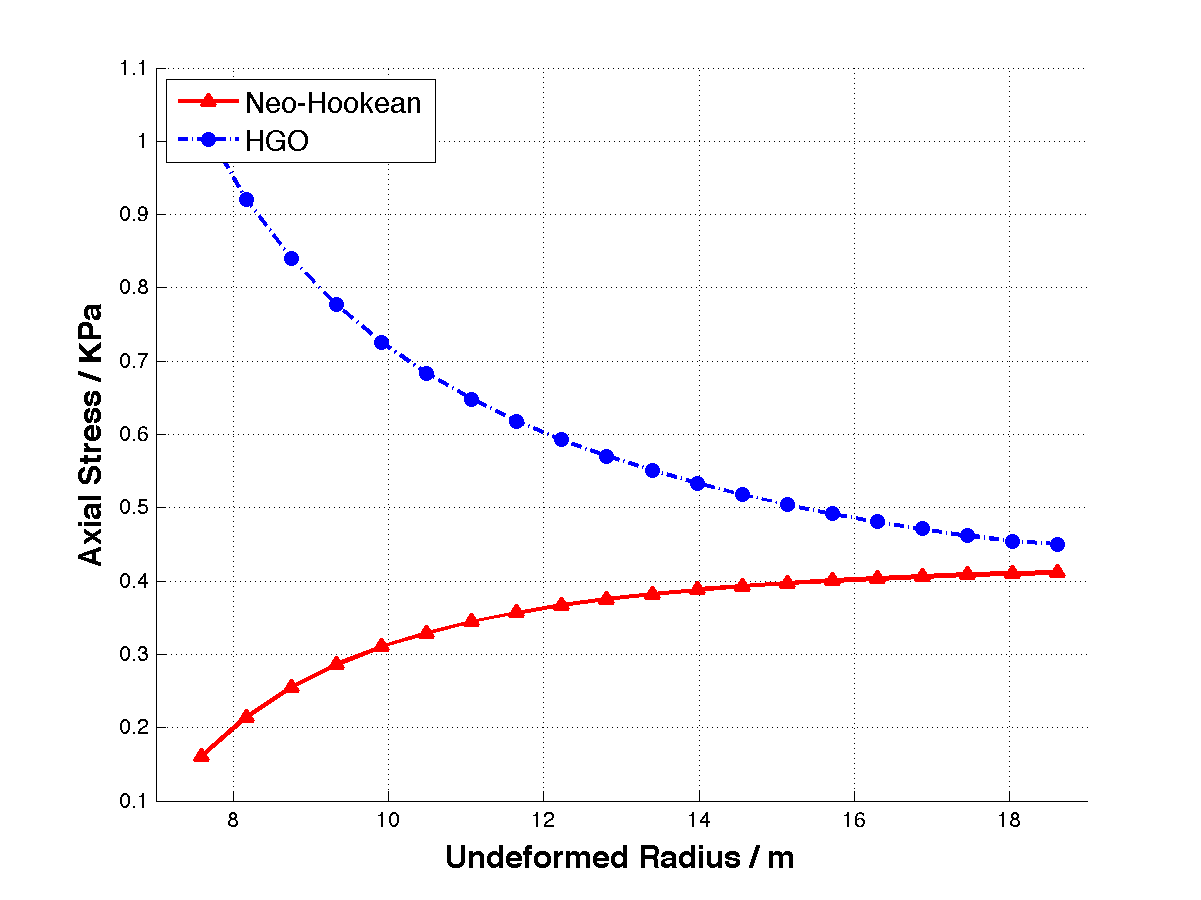
\includegraphics[width=\textwidth]{./figures/axial_nh_hgo.png}
		\caption{Axial Stress}
		\label{axial_nh_hgo}
	\end{subfigure}
	\caption{Vessel Expansion with Neo-Hookean and HGO Model under $1.5$ KPa}
	\label{fig:nh_hgo}
\end{figure}
















